\smalltitle{سوال 5}
\begin{enumerate}
    \item \begin{enumerate}
        \item تمام کد‌ها اعداد تصادفی یکسانی تولید می‌کنند (به علت \lr{srand(1)})
        و در تمامی آن‌ها صرفا تمام اعداد تصادفی را با هم جمع می‌زنیم.

        اما کمی تفاوت‌های جزئی وجود دارد. مثلا در فایل
        \lr{branch\_with\_true}
        صرفا شرط جمع یا ضرب در یک تابع جداگانه تعریف شده است که همیشه 1 را برگرداند. یا مثلا در فایل
        \lr{no\_branch}
        به صورت کلی شرط را برداشته‌ایم و همیشه جمع انجام می‌شود. در فایل
        \lr{real\_branch}
        باید دقت کنیم که خروجی تابع rand همیشه یک عدد مثبت است.
        پس تمامی اعداد آرایه برابر 1 هستند و شرط همیشه برقرار است.

        فرق این فایل با فایل اول این است که زمانی که کامپایلر می‌خواهد که کد را
        optimize
        بکند به کمک \lr{static analysis}
        نمی‌تواند شرط را حذف بکند و شرط همیشه وجود دارد.
        \item برای هر کدام از فایل‌ها دستور
        \lr{sudo perf stat ./*.out}
        را زدم. نتایج به صورت زیر هستند:
        \begin{latin}
        \begin{itemize}
            \item no\_branch.out
            \begin{figure}[H]
                \centerline{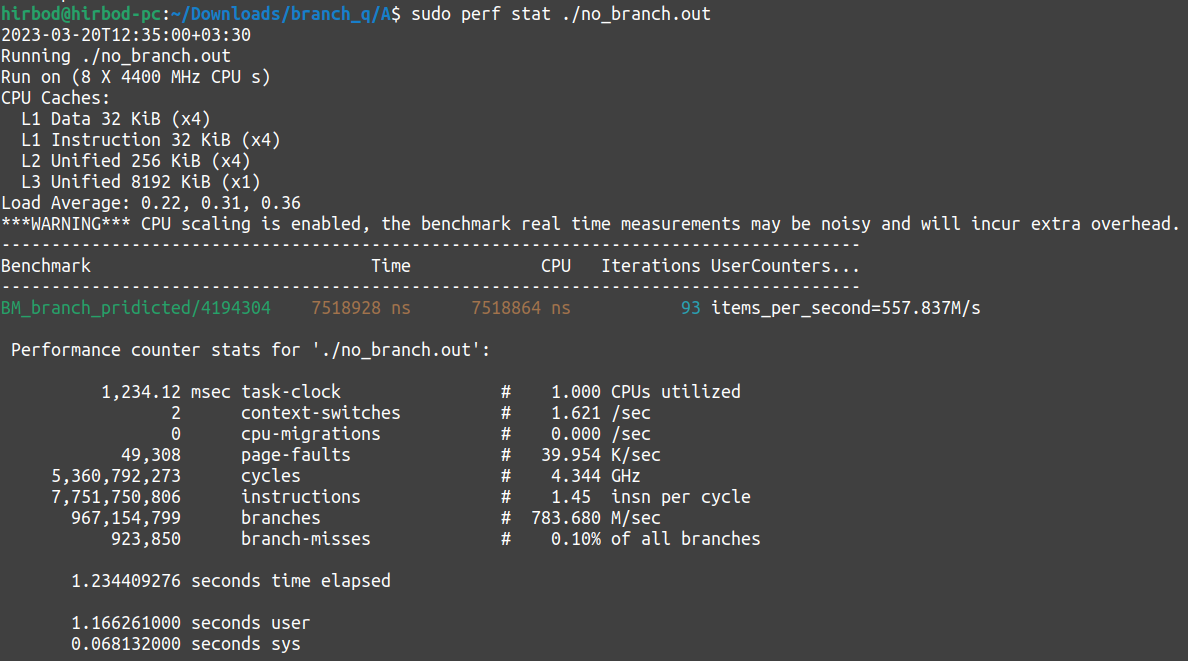
\includegraphics[scale=0.35]{pics/5/A/no_branch.png}}
            \end{figure}
            \item branch\_with\_true.out
            \begin{figure}[H]
                \centerline{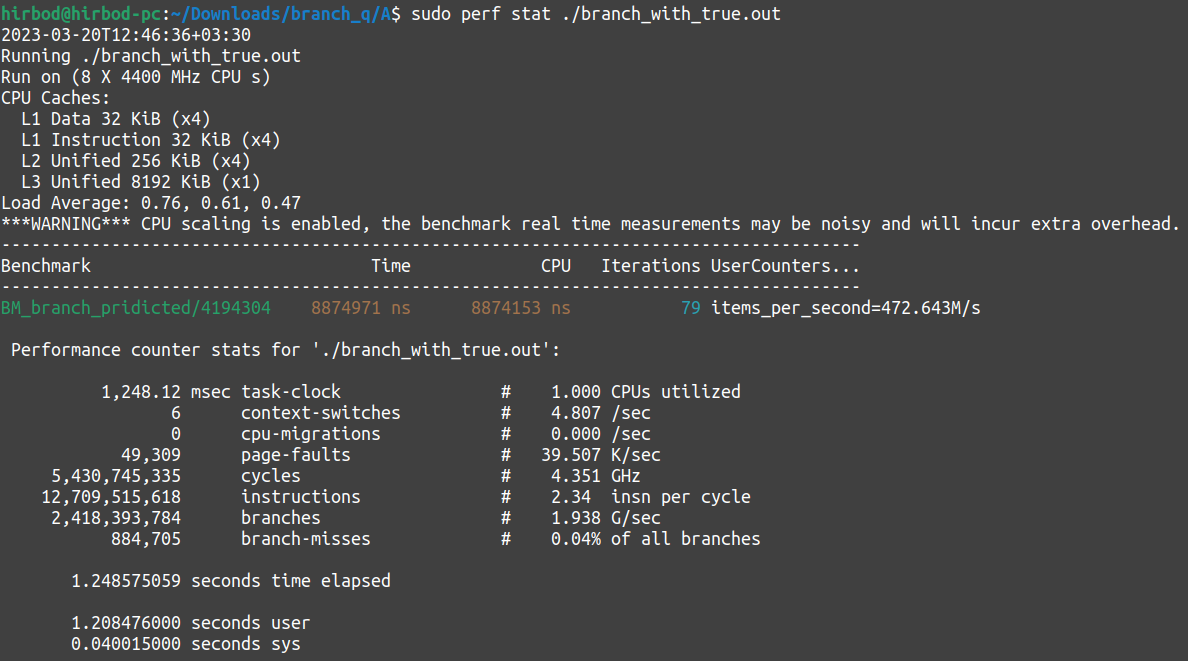
\includegraphics[scale=0.35]{pics/5/A/branch_with_true.png}}
            \end{figure}
            \item real\_branch.out
            \begin{figure}[H]
                \centerline{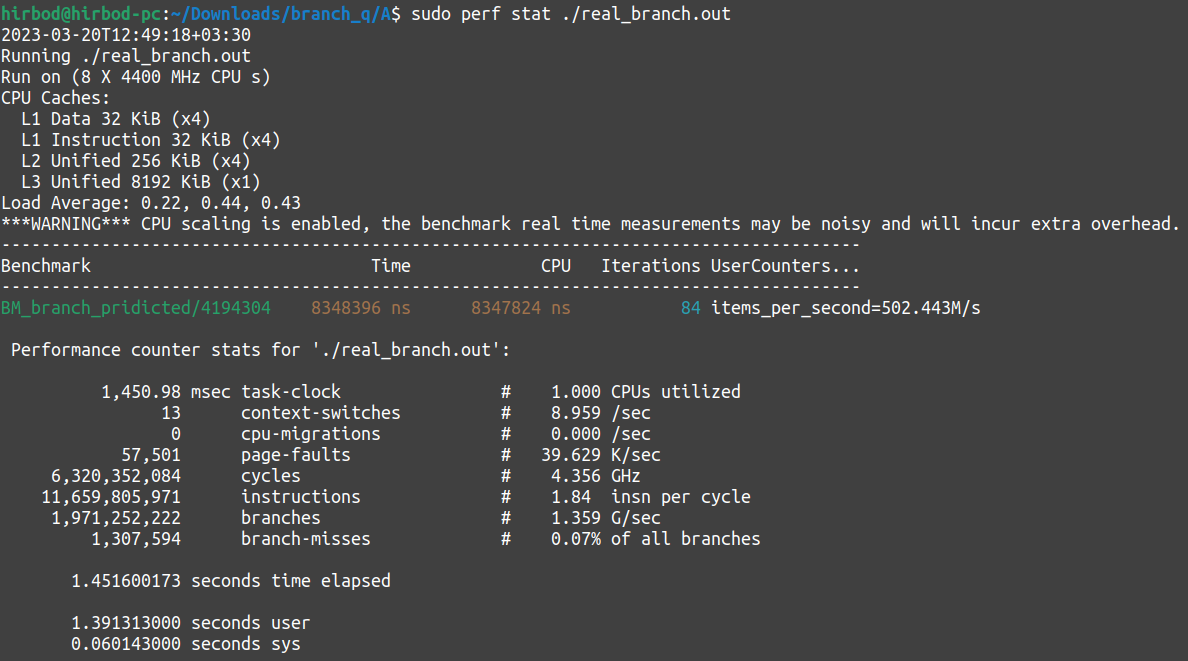
\includegraphics[scale=0.35]{pics/5/A/real_branch.png}}
            \end{figure}
        \end{itemize}
        \end{latin}
        همان طور که مشخص بود کدی که کلا branch ندارد سریع تر عمل می‌کند.
        اما کد‌هایی که branch دارند نیز به نسبت سریع هستند. همان طور که پیدا است به خاطر \lr{branch predictor cpu}
        است که این اتفاق می‌افتد. در صورتی که به نتایج perf نگاه کنیم متوجه می‌شویم که درصد خیلی کمی از
        \lr{branch}ها \lr{miss}
        شده‌اند. اما حال سوال پیش می‌آید که چرا
        \lr{branch\_with\_true}
        سریع‌تر از
        \lr{real\_branch}
        است. دلیل این موضوع را می‌توان در تعداد کل \lr{branch}ها
        مشاهده کرد. تعداد \lr{branch}های
        \lr{branch\_with\_true}
        بیشتر است. این اتفاق برای این می‌افتد که یک jump هم برای صدا زدن تابع \lr{true\_giver}
        و یک jump هم برای برگشت نیاز داریم.
        برای نگاه کردن به اسمبلی فایل من در ابتدا به کمک \lr{g++} \lr{object file}ها را ساختم و
        در ادامه به کمک
        \lr{ghidra}
        اسمبلی فایل‌ها را نگاه کردم. این اسمبلی برنامه‌ی
        \lr{brach\_with\_true}
        است:
        \begin{figure}[H]
            \centerline{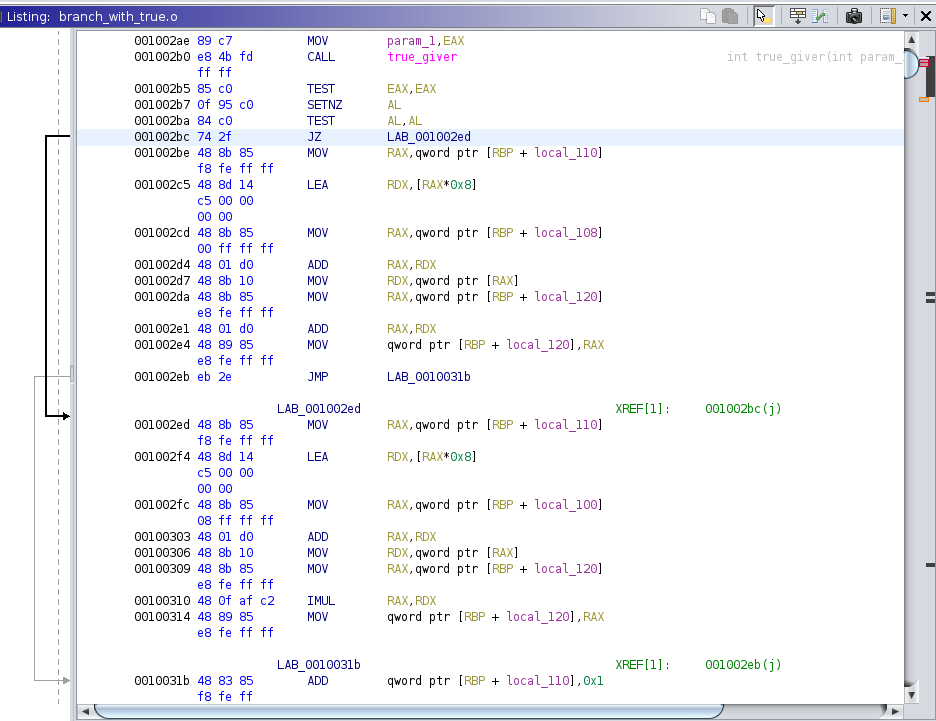
\includegraphics[scale=0.4]{pics/5/A/ghidra_branch_with_true.png}}
        \end{figure}
        و این نیز اسمبلی برنامه
        \lr{real\_branch}
        است:
        \begin{figure}[H]
            \centerline{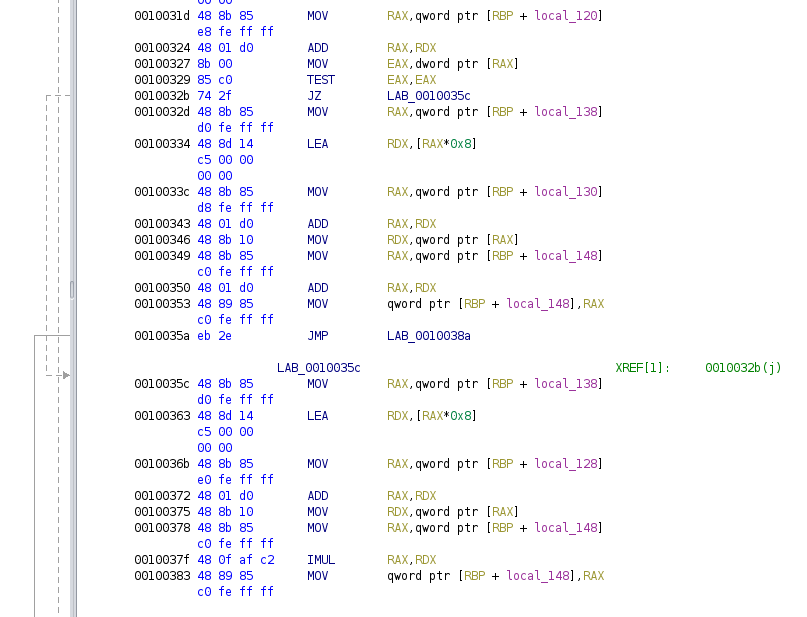
\includegraphics[scale=0.4]{pics/5/A/ghidra_real_branch.png}}
        \end{figure}
        همان طور که مشخص است تفاوت صرفا سر این است که یک call در برنامه‌ی \lr{branch\_with\_true}
        صورت گرفته است.
        \item در ابتدا صرفا هر کدام از برنامه‌ها را ران می‌کنیم:
        \begin{latin}
        \begin{itemize}
            \item no\_branch.O3
            \begin{figure}[H]
                \centerline{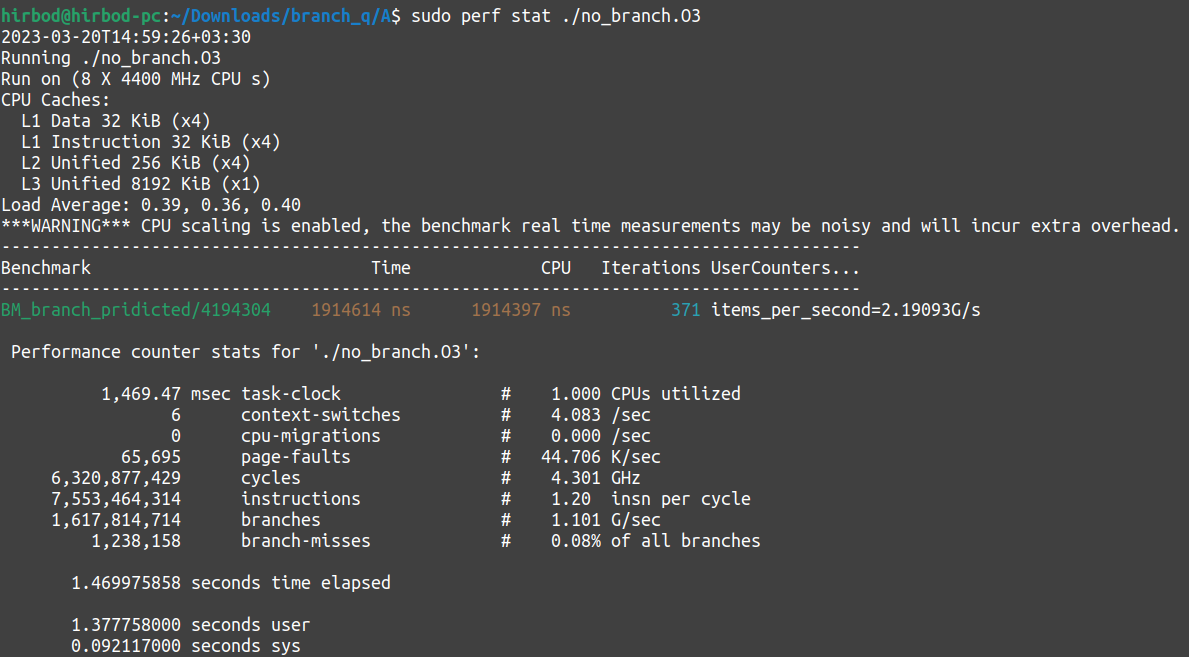
\includegraphics[scale=0.35]{pics/5/A/no_branch_o3.png}}
            \end{figure}
            \item branch\_with\_true.O3
            \begin{figure}[H]
                \centerline{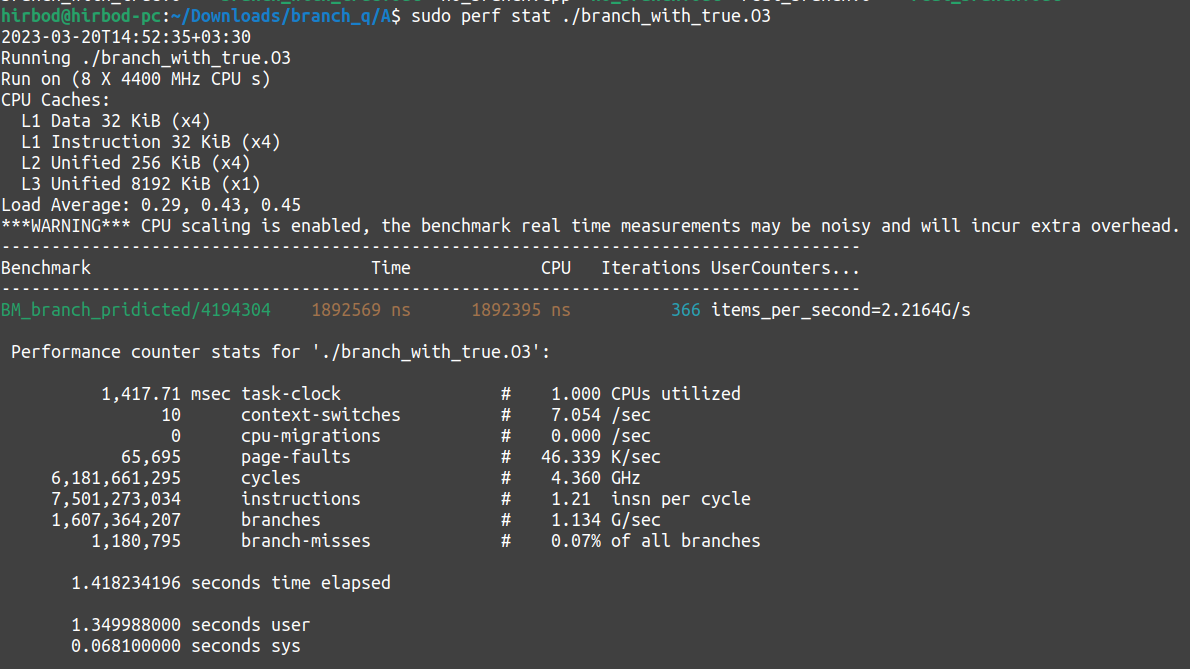
\includegraphics[scale=0.35]{pics/5/A/branch_with_true_o3.png}}
            \end{figure}
            \item real\_branch.O3
            \begin{figure}[H]
                \centerline{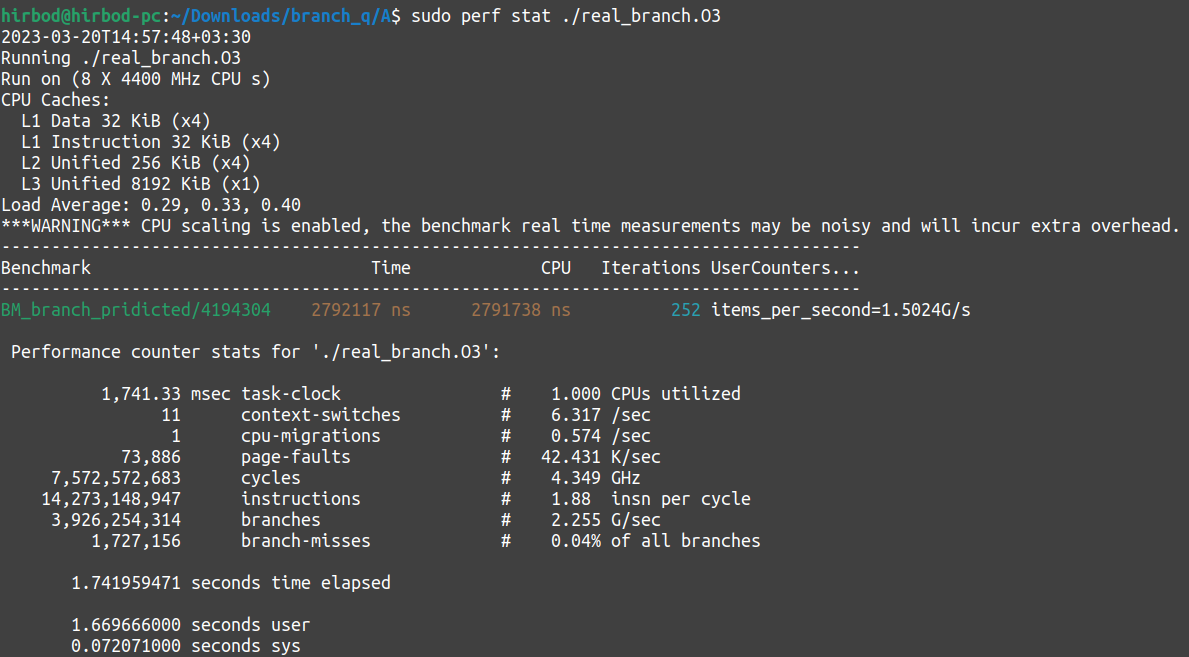
\includegraphics[scale=0.35]{pics/5/A/real_branch_o3.png}}
            \end{figure}
        \end{itemize}
        \end{latin}
        دلیل این موضوع این است که کامپایلر متوجه می‌شود که همیشه شرط موجود درست است و همیشه
        قطعه کد اول ران می‌شود. پس کامپایلر عملا شرط را بر می‌دارد و کد حاصل شبیه کد
        \lr{no\_branch}
        می‌شود. همان طور که در perf نیز مشخص است تعداد \lr{branch}ها تقریبا یکسان است.

        همچنین این تسریع سرعت را در \lr{real\_branch} نداشتیم چرا که در \lr{real\_branch}
        کامپایلر در زمان اجرا نمی‌تواند تشخیص دهد که آیا واقعا تمامی آرایه‌ی $c$
        برابر یک است یا خیر. برای همین هر دو قسمت شرط را قرار می‌دهد و یک branch اتفاق می‌افتد.
        این موضوع را می‌توان از خروجی perf نیز مشاهده کرد که تعداد \lr{branch}ها بسیار بیشتر از تعداد
        آنها در دو برنامه‌ی دیگر است.

        در نهایت نیز به کمک سایت
        \link{https://godbolt.org/}{godbolt}
        فرضیه‌ی خود را تست می‌کنیم.
        \begin{figure}[H]
            \centerline{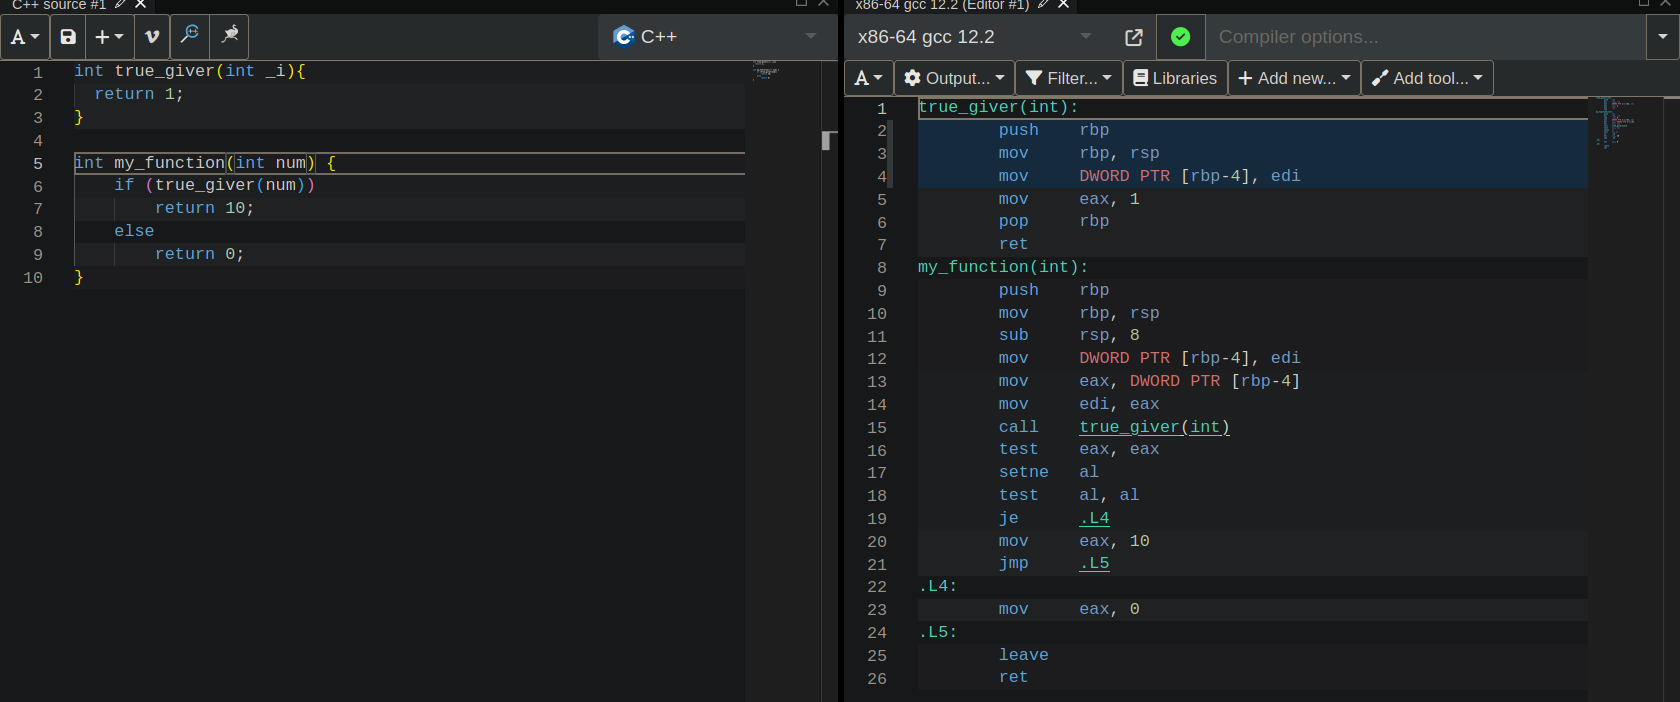
\includegraphics[scale=0.3]{pics/5/A/godbolt_o0.png}}
            \centerline{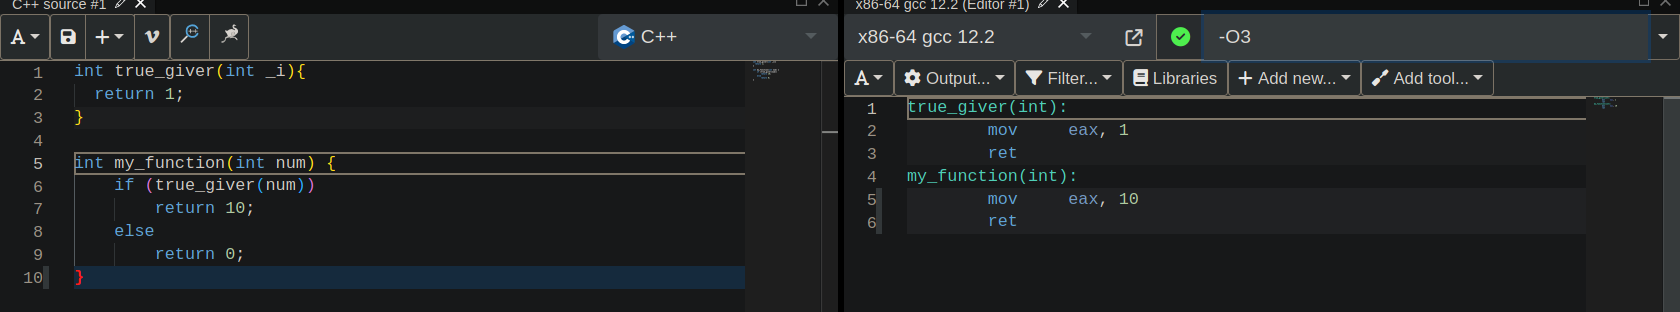
\includegraphics[scale=0.3]{pics/5/A/godbolt_o3.png}}
        \end{figure}
        همان طور که مشاهده می‌شود زمانی که از \lr{-O3}
        استفاده می‌کنیم به صورت کلی شرط برداشته می‌شود!
    \end{enumerate}
\end{enumerate}